\chapter{Discussion of Experimental Errors}
\label{Errors}
\section{Random Errors}
\subsection{Resolution of measurement}
The position of a detected particle is known to within a specified resolution, which translates into a resolution in the measurement of the opening angle between a pair of particles.
A particle's reconstructed position along a detector lengthwise is achieved by using the timing difference between two PMTs, producing a result known to within $\pm$13 cm.
Due to the detector's 15 cm width, there is also a positional uncertainty of $\pm 7.5$ cm in the direction perpendicular to the detector's length.
The amount of uncertainty in a two-neutron opening angle measurement is a function of the uncertainty in the positions of each neutron.
This function is determined by the propagation of the positional uncertainties through the formula for the calculation of opening angle, which is given by
\begin{displaymath}
    \theta_{nn} = \text{arccos}\left(\frac{\vec{v_{1}}^{\,}\cdot\vec{v_{2}}^{\,}}{|\vec{v_{1}}^{\,}||\vec{v_{2}}^{\,}|}\right)
\end{displaymath}
where $\vec{v_{1}}^{\,} = (x_1,y_1,z_1)$ and $\vec{v_{2}}^{\,} = (x_2,y_2,z_2)$ are the detected positions of the two neutrons.
The propagation of error through this formula is achieved by evaluating the following expression
\begin{eqnarray*}
\label{eq:propagation}
 \Delta \theta_{nn} & = & \left( \left(\Delta x_1 \frac{\partial \theta}{\partial x_1}\right)^{2} + \left(\Delta y_1 \frac{\partial \theta}{\partial y_1}\right)^{2} + \left(\Delta z_1 \frac{\partial \theta}{\partial z_1}\right)^{2} + \right. \\
 & & \left. + \left(\Delta x_2 \frac{\partial \theta}{\partial x_2}\right)^{2} + \left(\Delta y_2\frac{\partial \theta}{\partial y_2}\right)^{2} + \left(\Delta z_2 \frac{\partial \theta}{\partial z_2}\right)^{2} \right) ^{\frac{1}{2}}
\end{eqnarray*}
, where the $\Delta$'s represent the uncertainty in the variable that directly follows each $\Delta$.
The values and uncertainties of all events in a given angle bin are fed through Eq.\ref{eq:propagation}, and then averaged together.
The result, seen in fig~\ref{fig:OpeningAngleRes}, can be interpreted as the opening angle resolution as a function of $\theta$.
\begin{figure}[h]
    \centering
    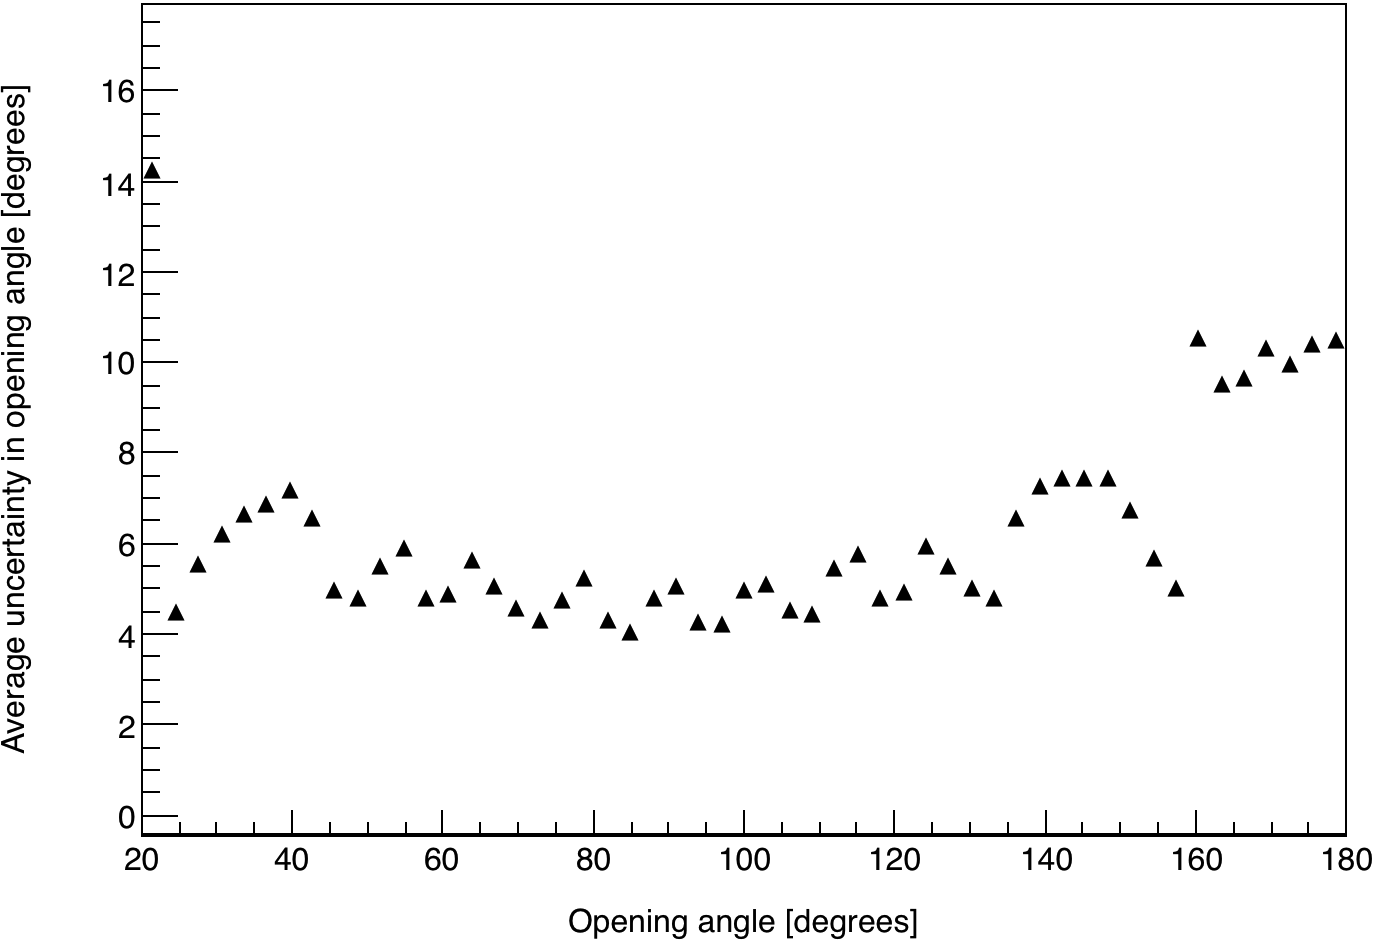
\includegraphics[width = 0.75\textwidth]{Content/Errors/OpeningAngleUncertainty.png}
    \caption{Uncertainties in opening angle determined by the propagation of position uncertainties through the opening angle calculation.
     The uncertainty of a given opening angle measurement depends on which detectors are involved and the position of the particles on the detectors.
     For this reason, the average uncertainty of measurements falling within each bin is taken.
    The y-axis can be viewed as a measure of the angular resolution in the sense that it represents the smallest angular difference that can be considered statistically significant.
    }
    \label{fig:OpeningAngleRes}
\end{figure}

\subsection{Counting error}
The uncertainty in the number of observed events is always assumed to be equal to $\sqrt{N}$, as per poissonian  statistics, were N is the number of observed events.
This value is propagated through all the analysis procedure using the standard method for the propagation of error.
The vertical error bars seen in all results are due solely to such counting error.

\FloatBarrier
\section{Detector Cross-talk}
\label{crosstalk}
\textit{Cross-talk} occurs when, after a particle is detected once, the same particle, by any means, causes a detection to be registered in a different detector.
For example, upon detection, a particle may undergo elastic scattering and then travel into a another detector where it is detected again, or it may produce secondary particles that are detected.
The two coincident detections forming a cross-talk event are causally correlated, and thus they have the potential to contaminate the signal from correlated fission neutrons.
If both detections occur during the ToF range typical for fission neutrons, then the cross-talk event cannot be distinguished from the detection of two correlated neutrons.

Recent works that measured the two-neutron angular correlations in the spontaneous fission of $^{252}$Cf and $^{240}$Pu~\cite{Pozzi2016,Verbeke2018} addressed this effect by using an MCNP-PoLiMi simulation to estimate and then subtract cross-talk from their measurements.
In this work, the issue of cross-talk is approached differently by employing the use of detector shielding aimed at reducing cross-talk to a negligible rate.
By using shielding to reduce cross-talk, this measurement is less dependent on the details of the models used by MCNP-PoLiMi to simulate neutron transport and detection.
MCNP-PoLoMi simulations are used in this work only to verify that the effect of cross-talk is negligible.
The scintillators used here are much larger than those used in similar works, such as in refs~\cite{Pozzi2016,Verbeke2018}, allowing for them to be placed much farther from the fission source without causing extremely low coincidence rates. 
An increase in the distance between the detectors and the fission source makes this measurement less sensitive to angular uncertainty, which is influenced by the uncertainty in the position of a detected particle, due to, for example, the scattering of neutrons from detector shielding.
Because of this, larger amounts of shielding can be used without concern of introducing large errors.

The geometry of the neutron detection system makes it kinematically impossible for a neutron to scatter from a proton in one detector--which is the basis for scintillation--and then travel directly into another detector with enough kinetic energy to be detected a second time.
For this reason, upon being detected, a neutron must scatter from one or more intermediate nuclei, such as Pb or C, in order for it to reach a different detector with enough energy to be detected a second time.
This fact follows from the conservation of energy and momentum.
Figure~\ref{fig:CrossTalkExample} illustrates a cross-talk event due to a neutron scattering in a detector's shielding.
In order to be convinced that such events occur at negligible rates, a detailed MCNP-PoliMi~\cite{MCNP_POLIMI} simulation was performed to model cross-talk.
\begin{figure}
    \centering
    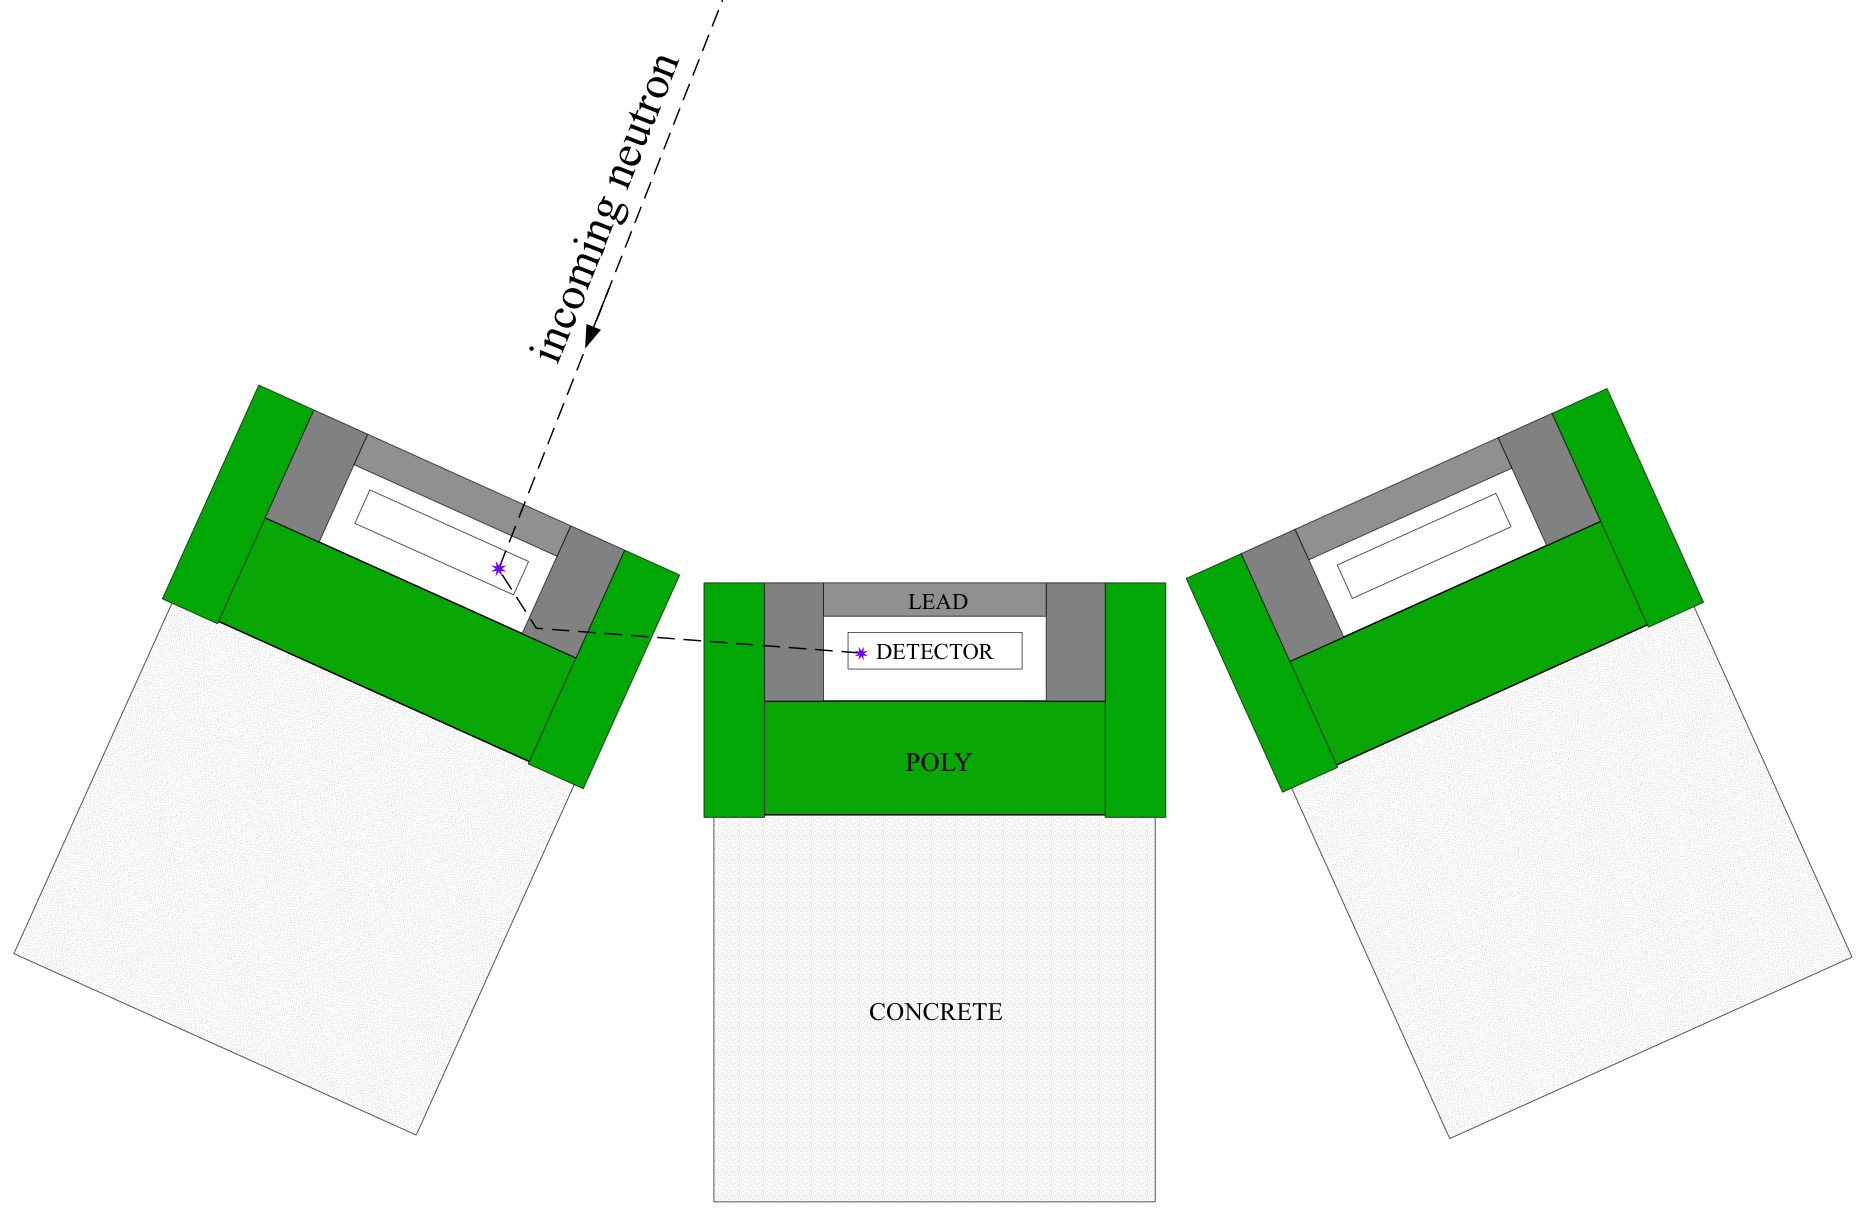
\includegraphics[width = 0.75\textwidth]{Content/Errors/CrossTalkExample.png}
    \caption{A hypothetical example of a neutron cross-talk event.
An incoming neutron detected and then scatters from some lead shielding nearby, which changes its direction of travel such that it enters a second detector where it is detected a second time.
The scattering of a neutron from an intermediate nucleus, in this case a lead nucleus, is kinematically required in order for cross-talk to occur in this experiment.}
    \label{fig:CrossTalkExample}
\end{figure}

\subsection{Cross-talk Simulation}
The simulation included all scintillators and their shielding, supporting structures, and the concrete walls surrounding the experimental cell.
MCNP-PoliMi's built-in $^{252}$Cf spontaneous fission source was used, which emits neutrons with the correct correlations and multiplicities.
Detector response was modeled using a program included with the MCNP-PoliMi distribution called MPPost~\cite{MPPost}.
The model is based on the electron equivalent light output (MeVee) produced by particles as they undergo collisions with carbon and hydrogen within organic plastic scintillators.
A minimum deposited energy of 0.4 MeV ( 0.05 MeVee for neutrons) was assumed for detectable particles, which was chosen because the neutron detection system showed a sharp decline in detection rates for neutrons below 0.4 MeV.
For neutron collisions with hydrogen, the light output in MeVee, $L$, is calculated by the following empirically derived formula
\begin{displaymath}
L = 0.0364 E_n^2 +  0.125 E_n
\end{displaymath}
where $E_n$ is equal to the loss in the kinetic energy of the neutron due to the collision.
Neutron interactions with carbon are assumed to generate a smal light output of
\begin{displaymath}
L = 0.02 E_n
\end{displaymath}
As seen in Fig.~\ref{fig:Cf252MCNPVsEXP}, the model produces a ToF spectrum that is in good agreement with the measurement.
\begin{figure}
    \centering
    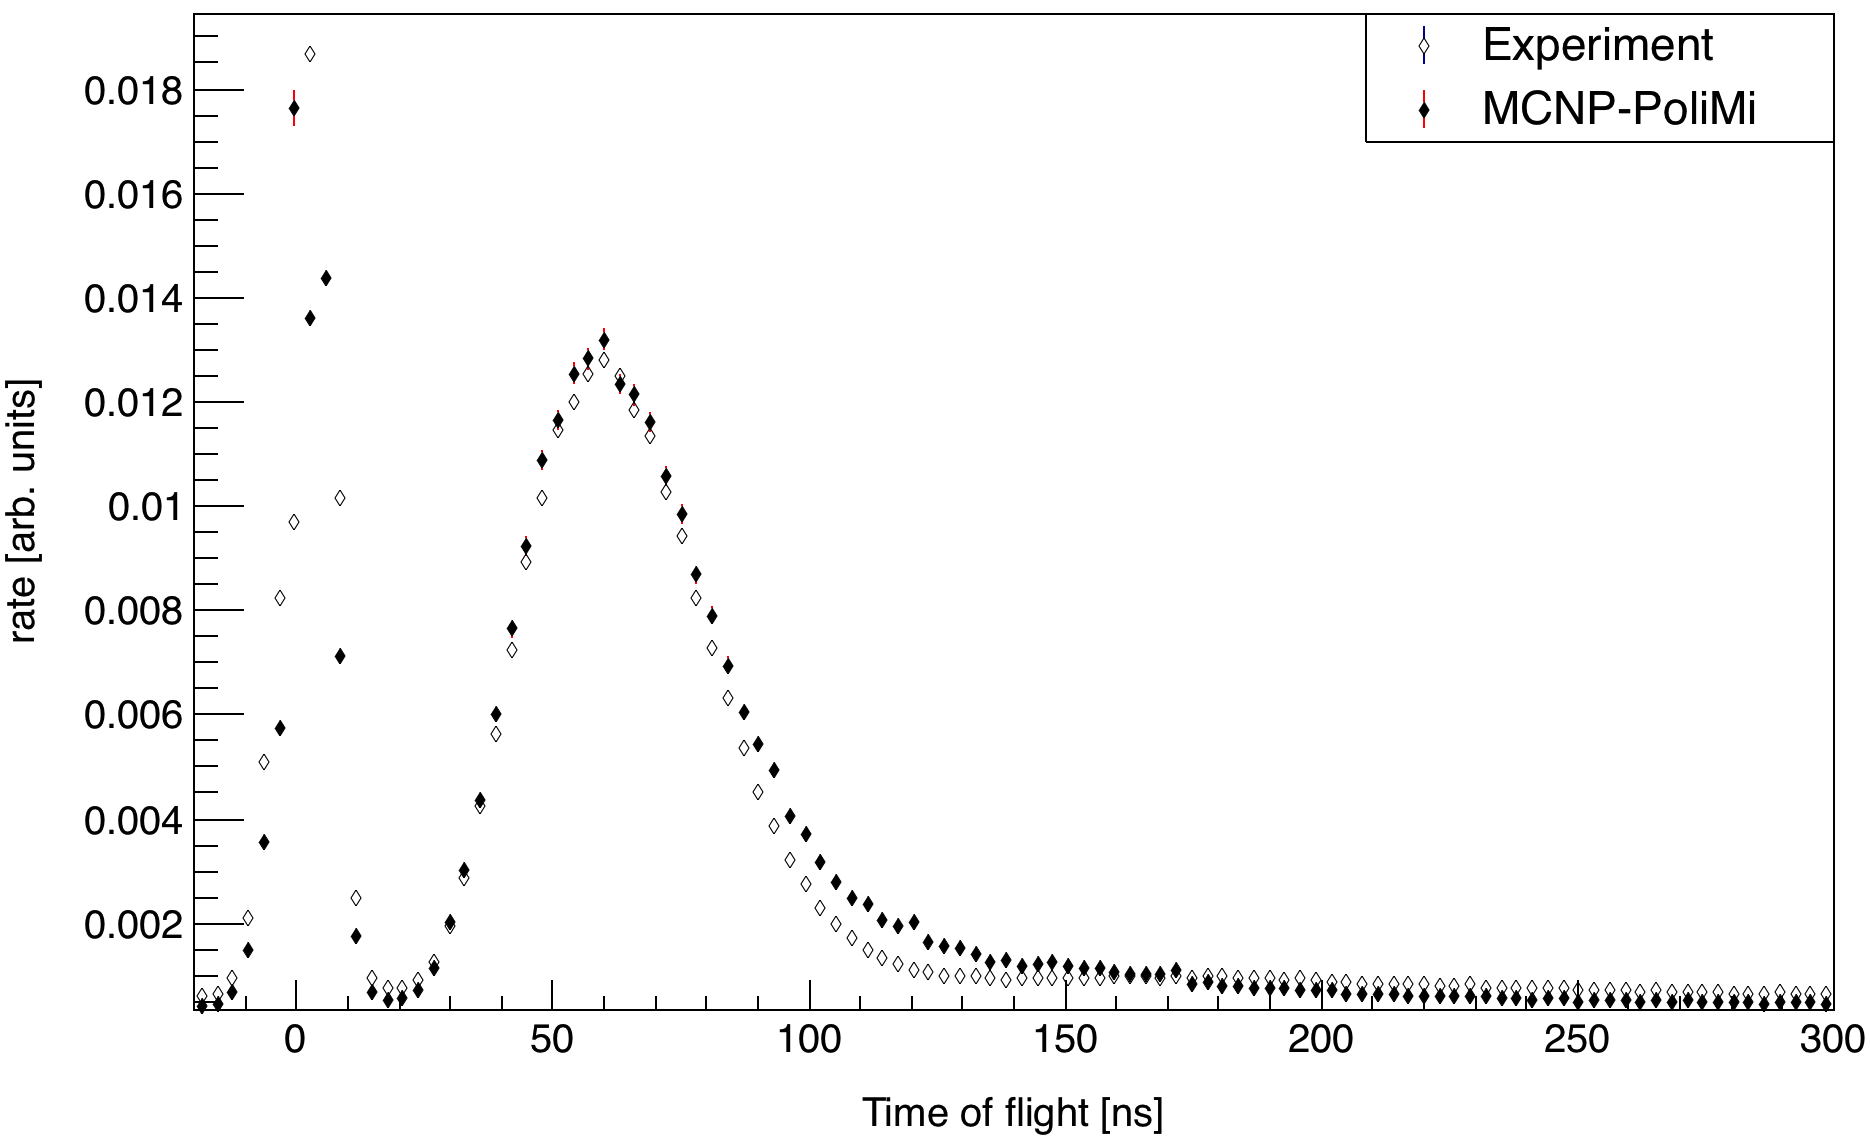
\includegraphics[width = 0.9\textwidth]{Content/Errors/Cf252MCNPVsEXP.png}
    \caption{Measured vs simulated ToF spectrum of a $^{252}$Cf spontaneous fission source.}
    \label{fig:Cf252MCNPVsEXP}
\end{figure}

The simulation was initially performed with 5 cm of lead shielding placed behind the scintillators, and the number of cross-talk events accounted for 11\% of the total coincident neutron events.
The amount of cross-talk fell to 3\% if polyethylene was used instead of lead to shield behind the detectors, which motivated the placement of 5 cm of polyethylene behind the detectors during construction.
Figure~\ref{fig:CrosstalkVScoincidence} shows the distribution of cross-talk events and true two-neutron coincidences as a function of reconstructed opening angle.
It is worth noting that, according to the simulation, the effect of cross-talk is not only small, but is also distributed over a wide range of angles rather than being concentrated around $\theta_{nn}=0$.
Angles greater than 125 degrees are not shown in Fig.~\ref{fig:CrosstalkVScoincidence}, because such events can be readily identified in analysis by the large amount of time required for the neutron to travel these distances.
\begin{figure}
    \centering
    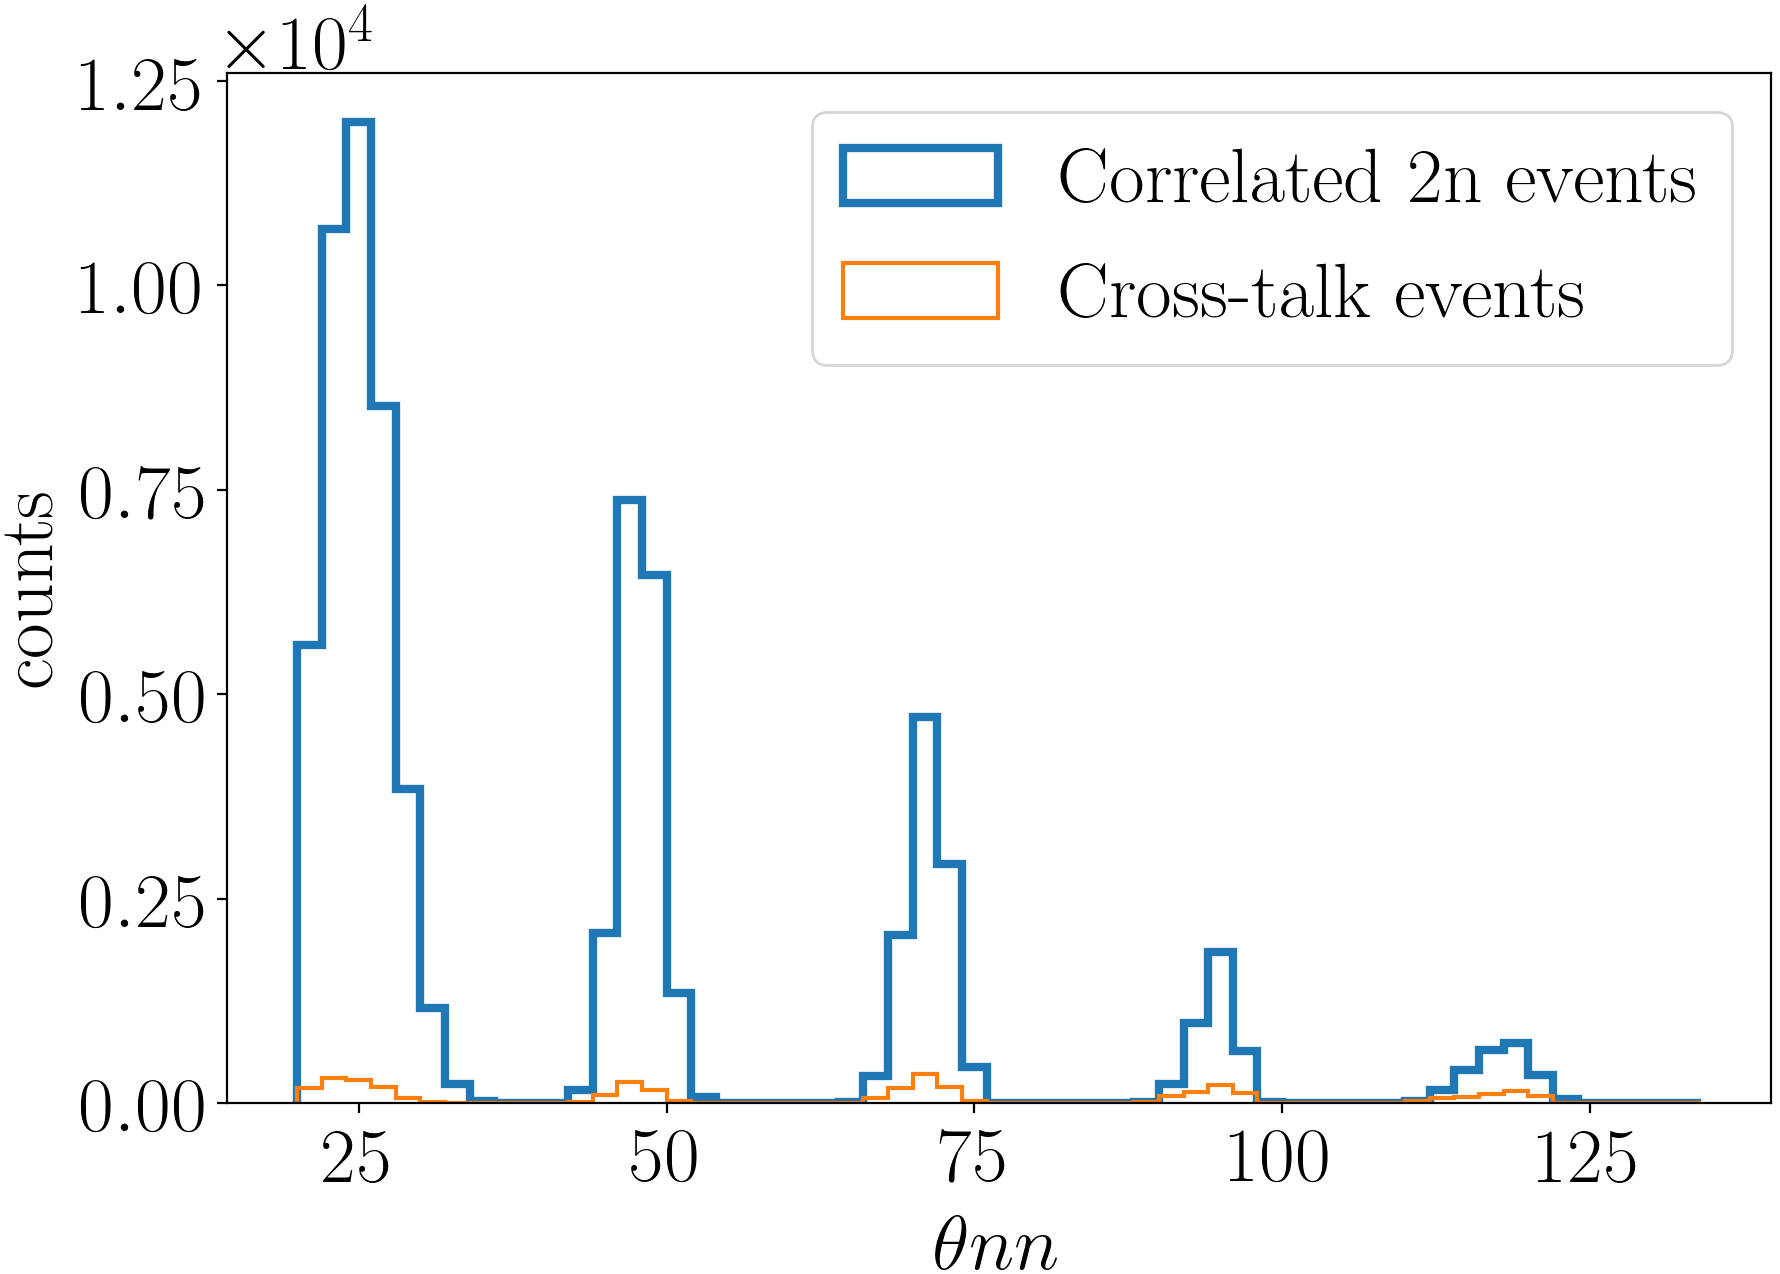
\includegraphics[width = 0.95\textwidth]{Content/Errors/CrosstalkVScoincidence.png}
    \caption{
    MCNP-PoLiMi simulation of the number of cross-talk events versus correlated two-neutron events as a function of reconstructed opening angle.
    Cross-talk accounted for 3\% of total events.
    In this work, cross-talk does not occur primarily at small angles, but is instead spread out over a wide range of angles.
    }
    \label{fig:CrosstalkVScoincidence}
\end{figure}

\subsection{Elastic Scattering in Target}
\label{subsection:Elastic_scattering}
A potential source of error in opening angle measurements is the scattering of neutrons within the fission target.
This is a cause for concern, because the scattering of neutrons from heavy nuclei highly alters the neutron's direction of travel, creating two-neutron opening angles that are not reflective of the true opening angle immediately after fission.
The target's dimensions are small enough that the rate of photon absorption, and thus photo-neutron production, is virtually uniform throughout the entire target volume.
MCNP was used to simulate the production of uncorrelated pairs of fission neutrons uniformly throughout the target volume, indicating that 5\% of neutron pairs undergo at least one scattering event between the two before they exit the target.

The chance that a neutron undergoes scattering within the target depends on how much target material the neutron travels through before exiting. 
This has the potential to create bias, because neutrons must travel through varying amounts of target material depending on which detector they reach.  
In particular, this could have an impact on measurements concerning the angle of neutrons with respect to the incoming photon beam.
In order to eliminate this problem, the target was rotated slowly about the vertical axis during data acquisition, creating a result equivalent to that if the target were actually a cylinder.
